\section{Démarche de Modélisation}
\subsection{Le robot poisson}

Le robot (robot poisson ou poisson) simulé est composé de 5 électrodes pour faire de l'\textit{électrolocation active}, c'est-à-dire pour générer un champ électrique qui réagit à l'environnement, tout comme le \textit{Gnathonemus petersii}. La suivante figure en deux dimension (le 5-ième capteur n'est pas représenté) montre le robot poisson simulé, ainsi que l'emplacement des électrodes. 

\begin{figure}[h!]
    \centering
    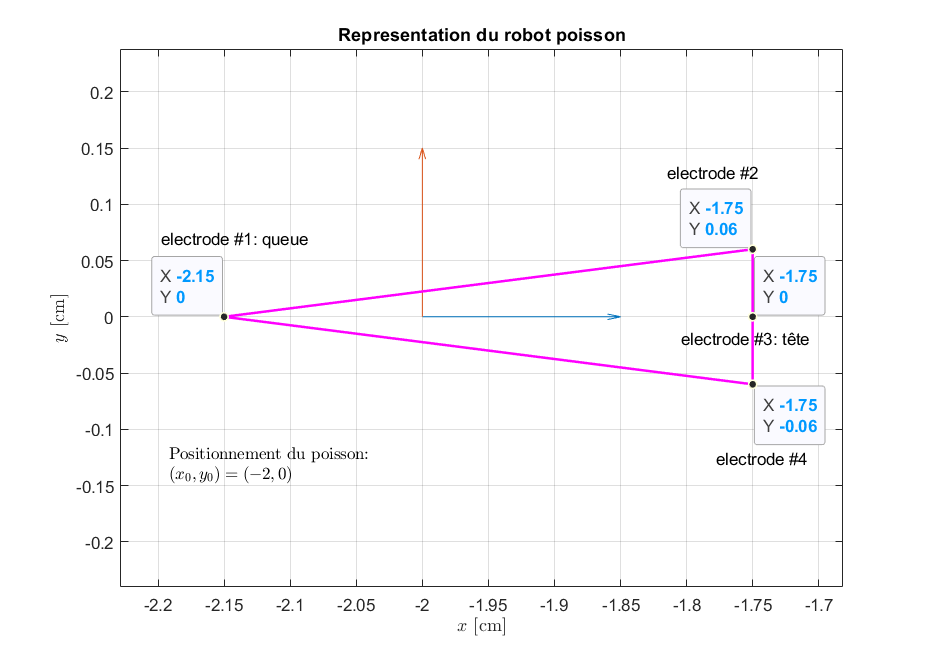
\includegraphics[width=\textwidth]{assets/poisson/poisson.png}
    \caption{Représentation du robot poisson et des capteurs dans le simulateur MATLAB}
    \label{fig:poisson}
\end{figure}

\subsection{La méthode des réflexions}
La méthode des réflexions est une solution au problème d'électrolocation directe, présentée sur \cite{Boyer2012}. Cette technique consiste à résoudre l'équation de Laplace $\Delta\phi = 0$ dans un scénario avec plusieurs objets autour du capteur et avec certaines conditions imposées aux objets (capteur inclus). En appliquant le principe de superposition présenté, nous pouvons résoudre l'équation de Laplace en considérant seulement les deux premières réflexions dans l'environnement du capteur et négligeant le reste des réflexions: nous tenons en compte donc l'émission du capteur $\phi_0$ en absence de tout objet, la réflexion de ce potentiel sur un objet et la seconde réflexion du potentiel émis par l'objet sur le capteur. La Figure \ref{fig:reflexions} résume bien le principe de cette méthode itérative. Chaque potentiel $\phi_i$ représente la réponse à la somme des potentiels $\phi_0 + \phi_1 + \dots \phi_{i-1}$ réfléchis par les objets qui entourent le capteur, et le capteur. Par conséquent, le problème se réduit à trouver les courants associés au potentiel de base $\phi_0$, la première et la seconde réflexion: $I^{(0)}, I^{(1)}$ et $I^{(2)}$. 
\clearpage 
\begin{figure}[h!]
    \centering
    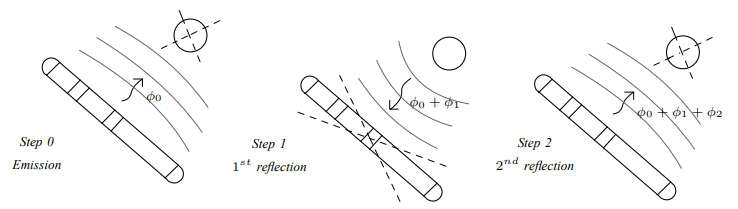
\includegraphics[width=0.8\textwidth]{doc/img/reflexions.png}
    \caption{Schéma des trois premières réflexions de la Méthode des Réflexions, image de \cite{Boyer2012}}
    \label{fig:reflexions}
\end{figure}

Le courant $I^{(0)}$ représente uniquement l'émetteur, il peut être obtenu en utilisant un simulateur numérique et s'écrit: 

\begin{equation}
    I^{(0)} = \bar{C}^{(0)} \cdot U
\end{equation}

avec $U$ étant le vecteur tension, dans notre cas $U = \left [1, 0, 0, 0, 0 \right ]$ car seulement l'électrode à la queue est alimenté, et $\bar{C}^{(0)}$ étant la matrice de conductances à vide entre chaque électrode et ayant la suivante forme dans notre cas: 
\begin{center}
$\bar{C}^{(0)} = \gamma \cdot 
\begin{pmatrix}
0.2557 & -0.0639 & -0.0639 & -0.0639 & -0.063 \\
-0.0639 & 0.1218 & -0.0203 & -0.0173 & -0.0203 \\
-0.0639 & -0.0203 & 0.1218 & -0.0203 & -0.0173 \\
-0.0639 & -0.0173 & -0.0203 & 0.1218 & -0.0203 \\
-0.0639 & -0.0203 & -0.0173 & -0.0203 & 0.1218 \\
\end{pmatrix}$
\end{center}

avec $\gamma$ la conductivité de l'eau $\left ( \text{en } \frac{S}{cm} \right )$.

Les courants $I^{(1)}$ et $I^{(2)}$ doivent être calculés en temps réel car ils dépendent de la position du capteur et du reste des objets. Nous divisons le courant généré par les réflexions en une composante axiale et une composante latérale. D'après \cite{Boyer2012}, \say{ la composante axiale $I_{\text{ax}}$ traduit la réaction du capteur aux différences de potentiel réfléchies par l'objet et évaluées le long de l'axe du capteur, et la composante latérale $I_{\text{lat}}$ traduit la polarisation latérale du capteur générée par le flux latéral du champ renvoyé par l'objet }: 

\begin{equation}
    I = I_{\text{ax}} + I_{\text{lat}}
\end{equation}
avec
\begin{equation}
    I_{\text{ax}} = \left ( 1- \bar{C}^{(0)} \cdot K \right ) \cdot P_{+} \cdot I^{(0)}
\end{equation}
et 
\begin{equation}
    I_{\text{lat}} = P_{\perp} \cdot L \cdot P_{+} \cdot I^{(0)}
\end{equation}

où, la matrice $P_{+}$ projette les courants à travers chaque électrode, en additionnant les courants de la même électrode, la matrice diagonale $P_{\perp}$ dépend de la géométrie du capteur, et les matrices $K$ et $L$ dépendent de la géométrie de l'objet et de sa position et orientation par rapport au capteur. 

Afin de simplifier le simulateur, nous allons négliger le courant latérale. En remplaçant le courant de base, le courant à étudier pour le contrôle du robot est de la forme: 

\begin{equation}
    I= \bar{C}^{(0)} \cdot U \left ( 1- \bar{C}^{(0)} \cdot K \right )
\end{equation}

Dans ce qui suit, nous devons calculer la matrice $K$ pour les différents objets que le capteur peut rencontrer. Nous allons considérer uniquement le cas d'un petit objet qui peut être isolant ou conducteur, et le cas d'un mur isolant. Notre simulateur placera des objets dans l'aquarium composé de 4 murs isolants. 
\newpage
\subsubsection{Cas d'un petit objet}
Pour le calcul de la matrice $K$ dans le cas d'un petit objet, nous prenons en compte le scénario composé d'un capteur (ou une électrode $\varepsilon_{\alpha}$), qui a pour centre $x_\alpha$, et d'un petit objet $\mathbf{p}$, qui lui a pour centre $y_c$.
\begin{figure}[h!]
    \centering
    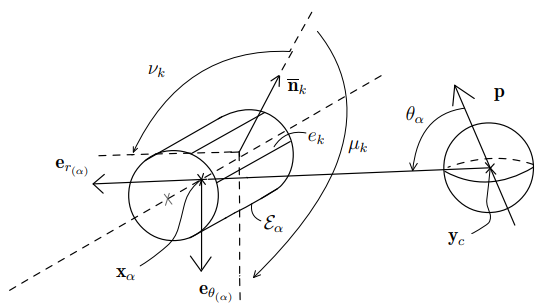
\includegraphics{doc/img/schema_petit_objet.png}
    \caption{Schéma représentant la macro-électrode $\varepsilon_{\alpha}$ du capteur perturbée par une sphère $\mathbf{p}$.}
    \label{fig:schema_petit_objet}
\end{figure}
Il est prouvé dans \cite{Boyer2012} que la matrice $K$ de réponse à cet objet suit l'expression suivante: 
\begin{equation}
    K = - \frac{1}{4\pi \cdot \gamma} \cdot \frac{r_\alpha \cdot P_r \cdot r_\beta}{\lVert r_\alpha \rVert^3 \cdot \lVert r_\beta \rVert^3}
\end{equation}
où, $r_\alpha = y_c - x_\alpha$, c'est-à-dire la distance entre l'objet et le capteur considéré, $r_\beta = y_c - x_\beta$, c'est-à-dire la distance entre l'objet et un autre capteur, et $P$ le tenseur de polarisation qui dépend de la géométrie de l'objet et du caractère conducteur/isolant. Pour une sphère, $P = \upchi \cdot a^3 \cdot I_{3}$ avec $I_3$ la matrice identité de $3$ dimensions, $a$ le rayon de la sphère et $\upchi$ le facteur de contraste: $1$ pour un objet totalement conducteur et $-0.5$ pour un objet totalement isolant.

Lors de la révision des résultats, vous trouverez la forme des courants lorsque le robot poisson traverse un objet totalement isolant et un objet totalement conducteur. 

\subsubsection{Cas d'un mur isolant}

Pour le cas des murs, nous utilisons la méthode présenté dans \cite{Jackson2012} pour des objets de grande taille. Comme illustré dans la Figure \ref{fig:schema_murs_coins}, cette méthode consiste à créer une image virtuelle du robot placée symétriquement au mur, qui a pour centre $x_\beta^*$ et, dans le cas d'approximation à un coin, une troisième image placée symétriquement au coin $C$. 

\begin{figure}[h!]
    \centering
    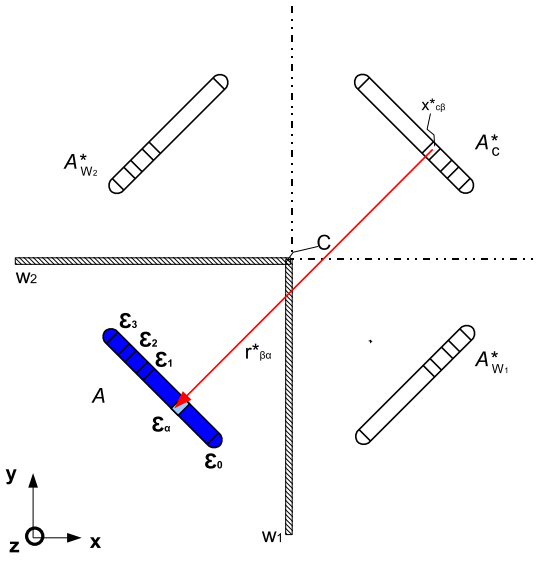
\includegraphics[scale=0.5]{doc/img/schema_murs_coins.png}
    \caption{Schéma représentant le capteur $A$ et les images virtuelles $A_{W_1}^*$ et $A_{W_2}^*$ symétriques aux murs $W_{1}$ et $W_{2}$, respectivement, et l'image virtuelle $A_C^*$ symétrique par rapport au coin $C$. }
    \label{fig:schema_murs_coins}
\end{figure}

En considérant le potentiel généré par le mur comme la superposition du champ du robot et le champ de son image, nous obtenons la matrice $K$ de réponse aux murs suivante: 

\begin{equation}
    K = - \frac{1}{4\pi \cdot \gamma} \cdot \frac{1}{\lVert r_{\beta\alpha}^* \rVert^3}
\end{equation}

où, $r_{\beta\alpha}^* = x_\alpha - x_\beta^*$ pour chaque combinaison d'électrode réel et électrode image. Du fait que notre aquarium porte 4 murs, nous avons 8 réflexions au total (4 réflexions provenant des murs et 4 réflexions provenant des coins). Dans la Figure \ref{fig:wall_reflexion} nous pouvons voir une représentation des 8 images virtuelles du robot poisson par rapport aux murs et aux coins. 

\begin{figure}
    \centering
    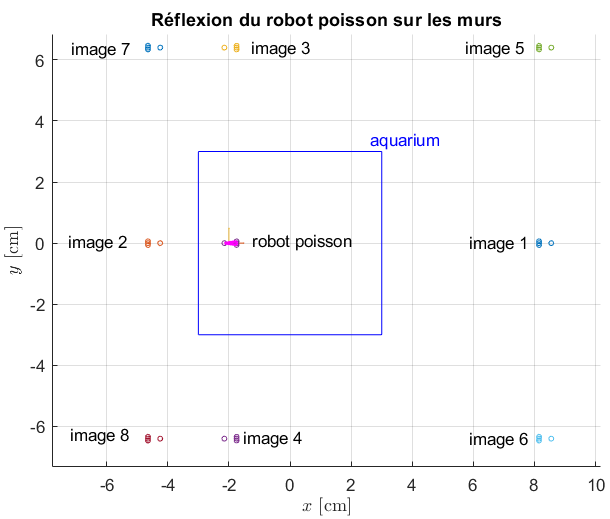
\includegraphics[scale=0.8]{assets/wall_reflexions/wall_reflexion.png}
    \caption{Réflexions du robot poisson par rapport aux murs et aux coins.}
    \label{fig:wall_reflexion}
\end{figure}
\clearpage

\subsection{Résultats obtenus}
Cette section montre les résultats obtenus lors de certaines simulations, qui permettent de valider le calcul des courants par Matlab. Dans le cas d'un petit objet isolant et conducteur, nous traversons l'objet et nous regardons les courants calculées. Dans le cas d'un mur isolant, nous regardons le courant lorsque le robot poisson s'approche au mur. 
\subsubsection{Cas d'un petit objet isolant}
\begin{figure}[h!]
    \centering
    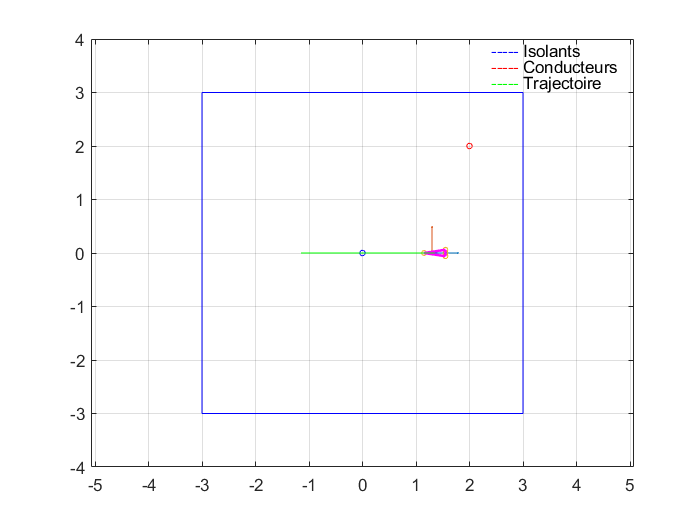
\includegraphics[width=0.5\textwidth]{assets/plot_currents/objet_isolant_2/objet_isolant_2_trajectoire.png}
    \caption{Représentation de l'aquarium pour la simulation. En bleu, les objets isolants (murs et objet), en rouge les objets conducteurs et en jaune la trajectoire suivi par le robot poisson.}
    \label{fig:objet_isolant_2_trajectoire}
\end{figure}
\begin{figure}[h!]
    \centering
    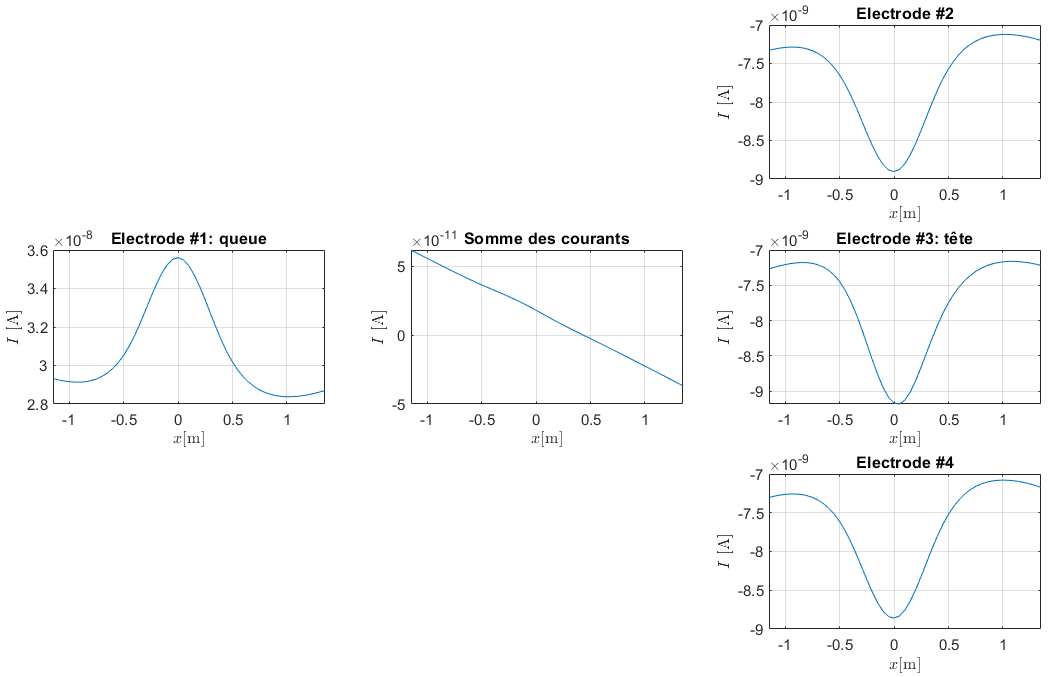
\includegraphics[width=0.9\textwidth]{assets/plot_currents/objet_isolant_2/objet_isolant_2.png}
    \caption{Courants obtenus dans l'électrode \#1 (queue), \#2, \#3 (tête) et \#4, lors de traverser un objet totalement isolant.}
    \label{fig:objet_isolant_2}
\end{figure}
\clearpage
\subsubsection{Cas d'un petit objet conducteur}
\begin{figure}[h!]
    \centering
    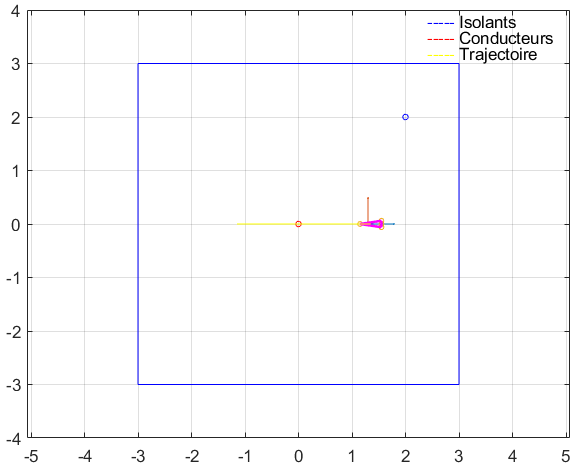
\includegraphics[width=0.5\textwidth]{assets/plot_currents/objet_conducteur_2/objet_conducteur_2_trajectoire.png}
    \caption{Représentation de l'aquarium pour la simulation. En bleu, les objets isolants (murs et objet), en rouge les objets conducteurs et en jaune la trajectoire suivi par le robot poisson.}
    \label{fig:objet_conducteur_2_trajectoire}
\end{figure}
\begin{figure}[h!]
    \centering
    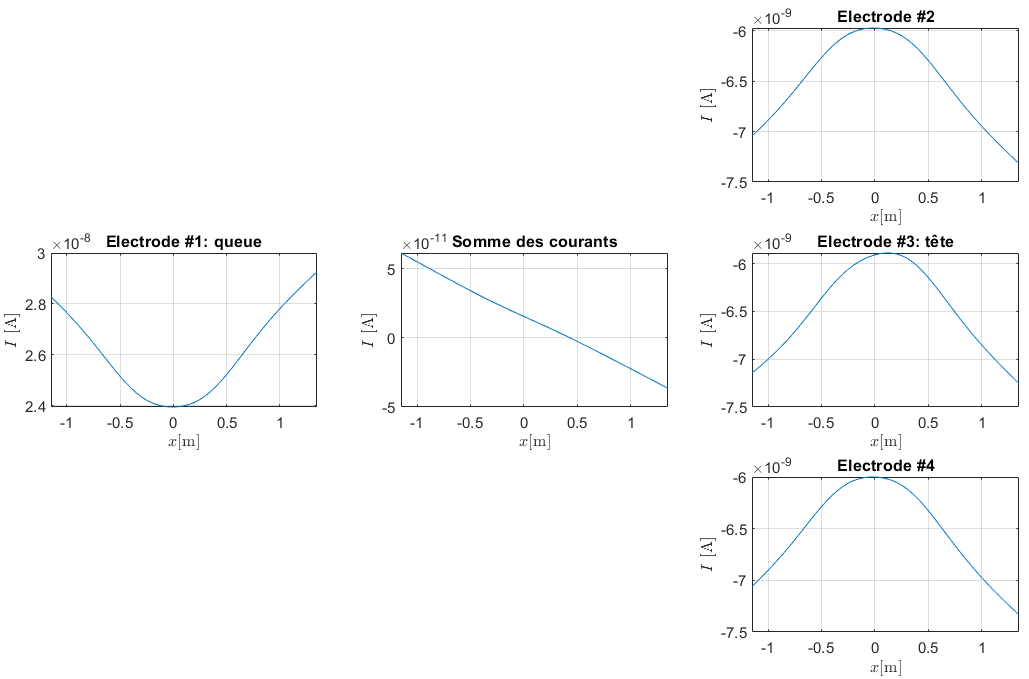
\includegraphics[width=0.9\textwidth]{assets/plot_currents/objet_conducteur_2/objet_conducteur_2.png}
    \caption{Courants obtenus dans l'électrode \#1 (queue), \#2, \#3 (tête) et \#4, lors de traverser un objet totalement conducteur.}
    \label{fig:objet_conducteur_2}
\end{figure}
\clearpage
\subsubsection{Cas d'un mur (isolant)}
\begin{figure}[h!]
    \centering
    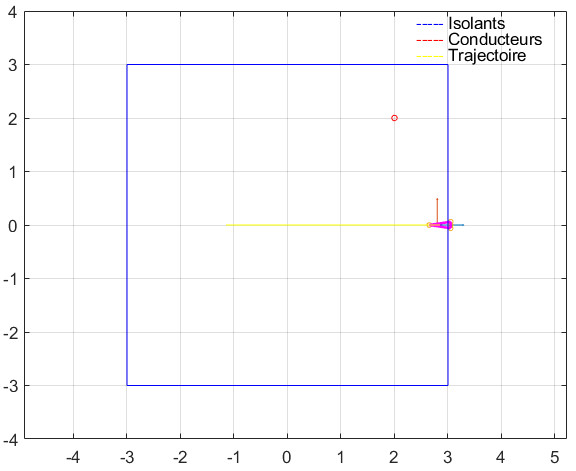
\includegraphics[width=0.5\textwidth]{assets/plot_currents/approximation_wall/approximation_wall_trajectoire.png}
    \caption{Représentation de l'aquarium pour la simulation. En bleu, les objets isolants (murs et objet), en rouge les objets conducteurs et en jaune la trajectoire suivi par le robot poisson.}
    \label{fig:approximation_wall_trajectoire}
\end{figure}
\begin{figure}[h!]
    \centering
    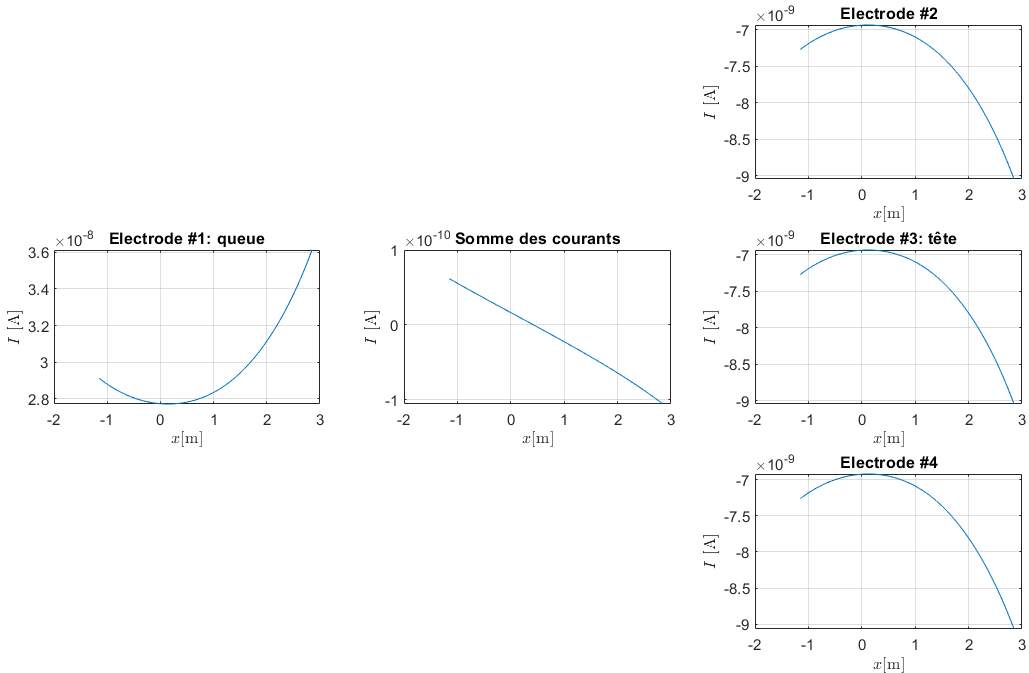
\includegraphics[width=0.9\textwidth]{assets/plot_currents/approximation_wall/approximation_wall.png}
    \caption{Courants obtenus dans l'électrode \#1 (queue), \#2, \#3 (tête) et \#4, lors de l'approximation à un mur.}
    \label{fig:approximation_wall}
\end{figure}